
\section{General Architecture}
\label{sec:architecture}


The goal of the re-developed HOPS architecture is provide a component-based design which allows for a greater degree of flexibility
in the types of operations that may be applied to VLBI data during fringe fitting, and avoid the semi-monolithic approach used in the past.
To do this, the software package to be delivered will primarily comprise of a set of loosely coupled libraries which can be composed
into an variety of calibration and fringe-fitting applications. Moreover, rather than attempting to identify and categorize all manner of data
types and data manipulation which may be required by future observations at the outset, a primary goal of this project is to provide a
relatively flexible set of data containers and operators along with a python plugin interface so as to allow for future extensions with minimal revision to the existing code.

For the foreseeable future, the main source of input data to this software will be provided by the DiFX correlator. However, this may not always
be the case, so in order to decouple the correlator from the post-processing software a conversion utility must be provided. This follows
the same paradigm as the current code, where a separate application (difx2mark4, which depends on the DIFXIO library) handles the conversion. However,
in this iteration we propose that this conversion utility operate mainly as a transparent pass-through, merely
converting the correlator output into the native post-processing data format, rather than applying any initial calibration/normalization (e.g. auto-corrs) or
other corrections to the data.

Once the data has been converted to the native post-processing format additional manipulation within the fringe-fitter will take place in several stages, such as normalization, data-flagging, a priori phase/delay and band-pass calibration, and finally fringe search. At intervening stages
both the data objects and data operator objects will be exposed to a python interface and hooks will be provided for external user scripts to 
access and directly modify the data and/or data operators. A extremely simplified diagram of the control flow of such a single-baseline fringe-fitter executable is shown in \ref{fig:fringe-fitter}. A multi-baseline global fringe-fitting algorithm will also be made possible by refactoring the HOPS code, however, the exact nature of this algorithm (e.g. Cotton-Schwab or baseline stacking, etc.) and whether it will best be implemented as a configurable option of a single fringe-fitting executable or as its own separate executable needs to be determine.

Upon completion of fringe fitting, the calibrated data with fringe solution applied will then be saved in a native binary format with the option to convert to an archival format (e.g. HDF5) via a simple conversion utility. Intermediate stages (with partial data corrections applied) may also optionally saved to the native format. It is also desired that
the export of a data flagging table and band-pass correction table be made possible, such an export tool may initially be implemented via user python script. If a multi-package (HOPS/AIPS/CASA) exchange format is adopted/specified then this feature could be made a built-in option in the refactored code.

In addition to the fringe fitter itself, a number of other post-fringing data analysis tools will also be provided. Most important are
a fringe plot utility for diagnostic information about the quality of an individual fringe, as well as the equivalent executables to \textit{alist} and \textit{aedit}, which summarize multiple fringe solutions and display condensed information about multiple scans respectively.
We intended to preserved the existing functionality of these executables, but expect to make the fringe-plot more flexible by providing options
to enable/disable various plotting items.


\begin{figure}[H]
\begin{center}
  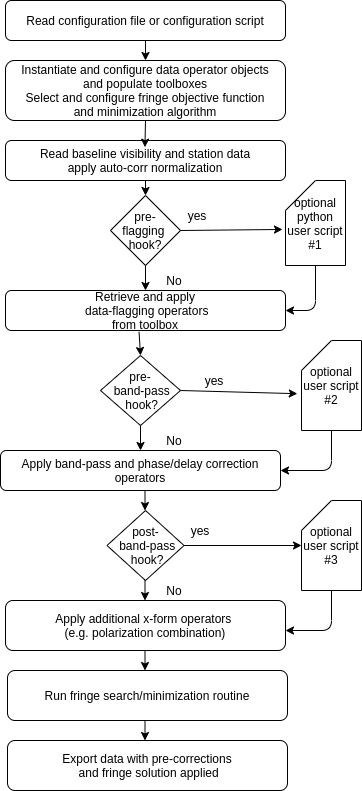
\includegraphics[width=0.6\textwidth]{fig/example-single-baseline-fringe-fitter.png}
    \caption{Example of simplified control flow for a single-baseline fringe fitter.}
    \label{fig:fringe-fitter}
\end{center}
\end{figure}


\section{The Visibility Data}

As mentioned in the previous section the primary output of the correlator are the ``visibilities'', which are essentially a two-dimensional array of complex values in time and frequency space. However, there are two details which were ignored in the preceeding section which are of importance in treating real data. 

The first detail is that most modern antennas record both electric field polarizations at once, producing four possible cross-correlation ``polarization-products'' for each baseline. Further complicating this is that the signals at each antenna may be recorded in a linear or circularly polarized basis, and so the ``polarization-products'' may be linear-linear, circular-circular or a mixed combination. Clearly delineating the polariation-product associated with the data is important, as a 
time-dependent phase and amplitude modulation can be introduced dpending on the telescope mount type and parallactic angle. We will leave a full discussion of this topic aside for the moment, but suffice to say that our single-baseline data set is extended in an additional ``polarization-product'' dimension.

The second complication is that we almost never deal with a single continuous chunk of bandwidth (i.e. a channel), but often have many channels distributed over a wider range of frequency. This done for several practical reasons. The first reason being that it is difficult to design RF systems that have a perfectly linear phase and amplitude response over a wide bandwidth. However, for narrow channels a linear phase/amplitude response is a perfectly reasonable approximation, and so linear corrections applied in a piecewise manner to several channels can be combined to simulat a flat bandpass over the full frequency range. The second reason (primarily of interest for geodesy) is that for a given recorded bandwidth, a better residual delay estimate can be obtained by spacing the recorded channels further apart in frequency than if they were entirely adjacent. Finally, channelized data
is also useful for RFI mitigation, since a narrow band RFI signal (provided it doesn't entirely saturate the frontend)
confined to a few channels can be easily deleted without having to edit the visibilities directly. While strictly speaking, a ``channel'' is simply shorthand for a frequency offset and thus not truly a separate dimension, for algorithmic considerations it is often convenient to treat this as if it were another independent axis over which the visibilities extend.

Therefore in order to accommodate multiple polarizations and channelization, our single-baseline visibility data generally is most easily represented as a uniform four dimensional array, indexed by polarization-product, channel, time (AP), and frequency (spectral point within a channel). This structure demands that each channel ought to contain the same number of spectral points,
and that each polariation-product ought to contain data for each channel and AP observed. It should be noted that this arrangement does come with some trade-offs between the overall memory usage and in efficiency of indexing across the data array. Ragged arrays would certainly be the most compact memory-wise, however they make random access very inefficient and are unlikely to be the most common use case and so are not considered as a general purpose container. In the occasional instances where channels may not share the same number of spectral points, it is expected that the deficient channels can be padded in order to maintain uniform spacing, or a non-channelized array 
can be used.

